\documentclass[tikz]{standalone}
    \usepackage{pgfplots}
    \pgfplotsset{compat=newest}
    \begin{document}
        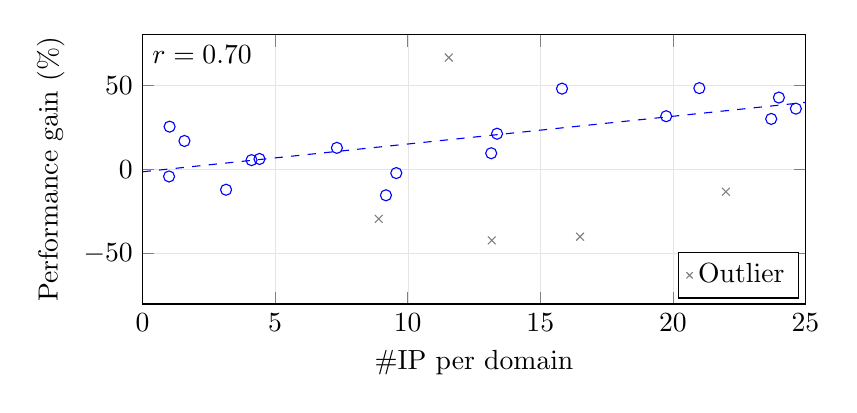
\begin{tikzpicture}[]
            \begin{axis}[%
                grid=both,
                grid style={line width=.1pt, draw=gray!20},
                xlabel={\#IP per domain},
                ylabel={Performance gain (\%)},
                width=10cm,
                height=5cm,
                ymin=-80,
                ymax=80,
                xmin=0,
                xmax=25,
                legend style={
                    at = {(.99,.02)},
                    anchor = south east
                },
                legend image post style={scale=0.8},
            ]
        \addplot[scatter, only marks, scatter src=explicit symbolic,
                  scatter/classes={
                      a={mark=o,draw=blue},
                      b={mark=x,draw=gray}
                  }]
        table[x=x,y=y,meta=label] {
        x y label
        15.82 48.0 a
13.15 9.6 a
19.75 31.6 a
24.64 36.1 a
9.18 -15.4 a
3.15 -12.1 a
8.91 -29.4 b
9.57 -2.1999999999999997 a
7.33 12.8 a
4.11 5.5 a
24.0 42.699999999999996 a
21.0 48.3 a
13.17 -42.199999999999996 b
22.0 -13.3 b
1.0 -4.2 a
23.71 30.0 a
1.58 16.900000000000002 a
16.5 -40.0 b
11.55 66.5 b
1.02 25.4 a
4.41 6.2 a
13.37 21.2 a
        };
        \legend{,Outlier}
        \addplot+[blue, dashed, mark=none] coordinates {(0,-1.42) (26,41.46)};
        \addplot+[black, mark=none] coordinates{(0, 68)} node[midway,right]{$r = 0.70$};
        \end{axis}
        \end{tikzpicture}
    \end{document}
